\documentclass{magnolia}

\magtex{tex_driver={pdftex}}
\magfiche{document_nom={Représentation des données},
          auteur_nom={François Fayard},
          auteur_mail={francois.fayard@auxlazaristeslasalle.fr}}
\magexos{exos_matiere={maths},
         exos_niveau={mpsi},
         exos_chapitre_numero={1},
         exos_theme={Représentation des données}}
\magmisenpage{}
\maglieudiff{}
\magprocess

\begin{document}

%BEGIN_BOOK

\magsection{Les entiers}
\magsubsection{Décomposition en base $b$}

\exercice{nom={Calculs en base 2}}
Réaliser les opérations suivantes en base 2, sans passer par la base 10, à l'aide des
algorithmes appris à l'école primaire.
\[\underline{101010}_2+\underline{11000}_2\qsep \underline{110101}_2-\underline{11001}_2\qsep \underline{11101}_2 \times \underline{1011}_2\qsep
  \underline{1100101}_2 / \underline{1011}_2.\]


\exercice{nom={Somme et produit en base $b$}}
Dans cet exercice, un entier $d\in\N$ est représenté par sa décomposition en base
$b\geq 2$, c'est-à-dire par une liste d'entiers $d_k\in\interefo{0}{b}$ pour $0\leq k<n$,
telle que
\[d=\sum_{k=0}^{n-1} d_k b^k.\]
Les chiffres de poids faible sont situés en début de liste alors que les chiffres
de poids fort sont quant à eux en fin de liste.  Le but de cet exercice est
d'implémenter l'addition et la multiplication en base $b$, comme on l'a appris à l'école
primaire.
\begin{questions}
% \question Montrer que lors de l'addition de deux nombres $d$ et $e$ en base $b$,
%   à chaque étape, la retenue est soit égale à 0, soit égale à 1.
\question Écrire une fonction \verb!chiffre(d: list[int], k: int) -> int! renvoyant
  le chiffre $d_k$ du nombre $d$. Si $k$ est plus grand que la longueur de
  la liste \verb!d!, cette fonction devra renvoyer 0.
\question Écrire une fonction
  \verb!addition(d: list[int], e: list[int], b: int) -> list[int]! réalisant l'addition
  de deux nombres $d$ et $e$ en base $b$.
\question
\begin{questions}
% \question Montrer que lors de la multiplication d'un nombre $d\in\N$ en base $b$ par
%   un chiffre $c\in\interefo{0}{b}$, la retenue est toujours dans $\interefo{0}{b}$. 
\question Écrire une fonction
  \verb!multiplication_chiffre(d: list[int], c: int, i: int, b: int) -> list[int]!
  réalisant la multiplication en base $b$ du nombre $d\in\N$ par $c b^i$, où
  $c\in\interefo{0}{b}$ et $i\in\N$.
\question En déduire la fonction \verb!multiplication(d: list[int], e: list[int], b: int) -> list[int]!
  réalisant la multiplication de deux nombres $d$ et $e$ en base $b$. 
\end{questions}
\end{questions}

\exercice{nom={Incrément binaire}}
Écrire une fonction \verb!increment(d: list[int]) -> NoneType! prenant en entrée la
décomposition binaire
\[d=\sum_{k=0}^{n-1} d_k 2^k\]
du nombre $d$ et la transformant en celle de $d+1$.


\exercice{nom={Espace binaire}}
On appelle espace binaire d'un entier naturel $n$ toute séquence consécutive de 0 délimités
par deux 1 dans la décomposition en base 2 de $n$. Par exemple, le nombre 529 possède deux
espaces binaires de longueurs respectives 3 et 4 car $529=\underline{1000010001}_2$. En revanche, 32 ne
possède pas d'espace binaire puisque $32=\underline{100000}_2$.\\

Écrire une fonction \verb!espace_binaire(n: int) -> int! qui prend pour argument un entier naturel
et renvoie la longueur du plus grand espace binaire présent dans $n$ s'il existe, et la valeur
0 sinon.


\exercice{nom={Factorion}}
On appelle factorion, tout entier naturel qui est égal à la somme des factorielles de
ses chiffres. Par exemple, 145 est un factorion en écriture décimale, car
\[1! + 4! + 5! = 1 + 24 + 120 = 125.\]
\begin{questions}
\question Écrire une fonction \verb!factorielle(n : int) -> int!, calculant la
  factorielle d'un entier $n$.
\question Écrire une fonction \verb!factorion(m: int, b: int) -> bool!, déterminant
  si $m$ est un factorion en base $b$.
\question En déduire une fonction \verb!liste_factorions(b: int, p:int) -> list[int]!,
  renvoyant l'ensemble des factorions inférieurs ou égaux à $p$. 
\question
\begin{questions}
\question Montrer que si $m\in\N$ est un factorion de $n$ chiffres en base $b$, alors
  \[b^{n-1} \leq m \leq n(b-1)!.\]
\emph{En particulier, si
  \[u_n \defeq \frac{n(b-1)!}{b^{n-1}}<1,\]
  alors il n'existe aucun factorion de $n$ chiffres.}
\question Montrer que la suite $(u_n)$ est décroissante et tend vers 0,
  puis écrire une fonction
\begin{center}
  \verb!les_factorions(b: int) -> list[int]!
\end{center}
  renvoyant l'ensemble des factorions en base $b$.
\end{questions}
\end{questions}

\exercice{nom={Toblerone}}
Après un changement de l'équipe dirigeante, l'entreprise Mondelez
International, qui fabrique les barres Toblerone, décide de rationaliser
sa production pour maximiser ses revenus. En effet, leur chaine de production
fabrique des barres de $n$ «~carreaux~» qui sont ensuite coupées en barres plus
petites avant d'être vendues. Mais une récente étude de marché a déterminé le
prix auquel on pouvait vendre des barres de longueur $k$ (pour
$0 \leq k \leq n$), et ce prix s'avère ne pas avoir de relation simple avec $k$.
Le problème est donc de décider comment découper la barre initiale de $n$
carreaux en des barres plus petites pour maximiser le prix de vente total.\\

Dans tout le problème, on considèrera que l'on dispose d'un tableau
\verb!p!, indicé de $0$ à $n$, tel que \verb!p[k]! est le prix de
vente d'une barre de longueur $k$. Bien entendu, le prix d'un morceau de taille 0
est 0. Remarquez que si \verb!p[n]! est suffisamment grand, la solution optimale peut
très bien être de ne pas découper la barre.

\begin{center}
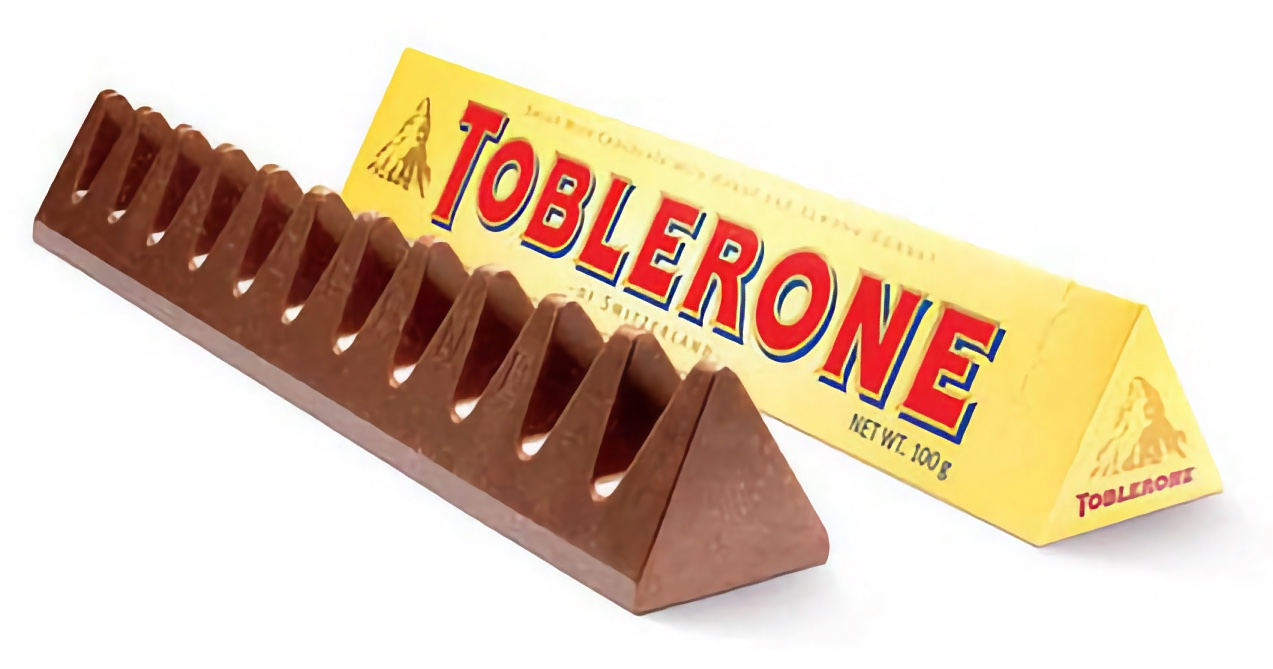
\includegraphics[width=0.5\textwidth]{../../Commun/Images/python-exos-toblerone}
\end{center}

\noindent On donne un exemple de tableau $p$ pour $n = 10$.
\begin{center}
  \begin{tabular}{r *{11}{c}}
    \toprule
    $k$   & 0 & 1 & 2 & 3 & 4 & 5 & 6 & 7 & 8 & 9 & 10\\
    \midrule
    ${p_k}$ & 0 & 1 & 5 & 8 & 9 & 10& 17& 17 & 20& 24& 26 \\
    \bottomrule
  \end{tabular}
\end{center}

Pour résoudre ce problème, on commence par établir une correspondance entre
les découpes d'un Toblerone composé de $n$ carreaux et les tableaux $d$
de $n-1$ booléens~: on coupe après le carreau d'indice $k$ si et seulement si
$d_k$ est vrai.

\begin{center}
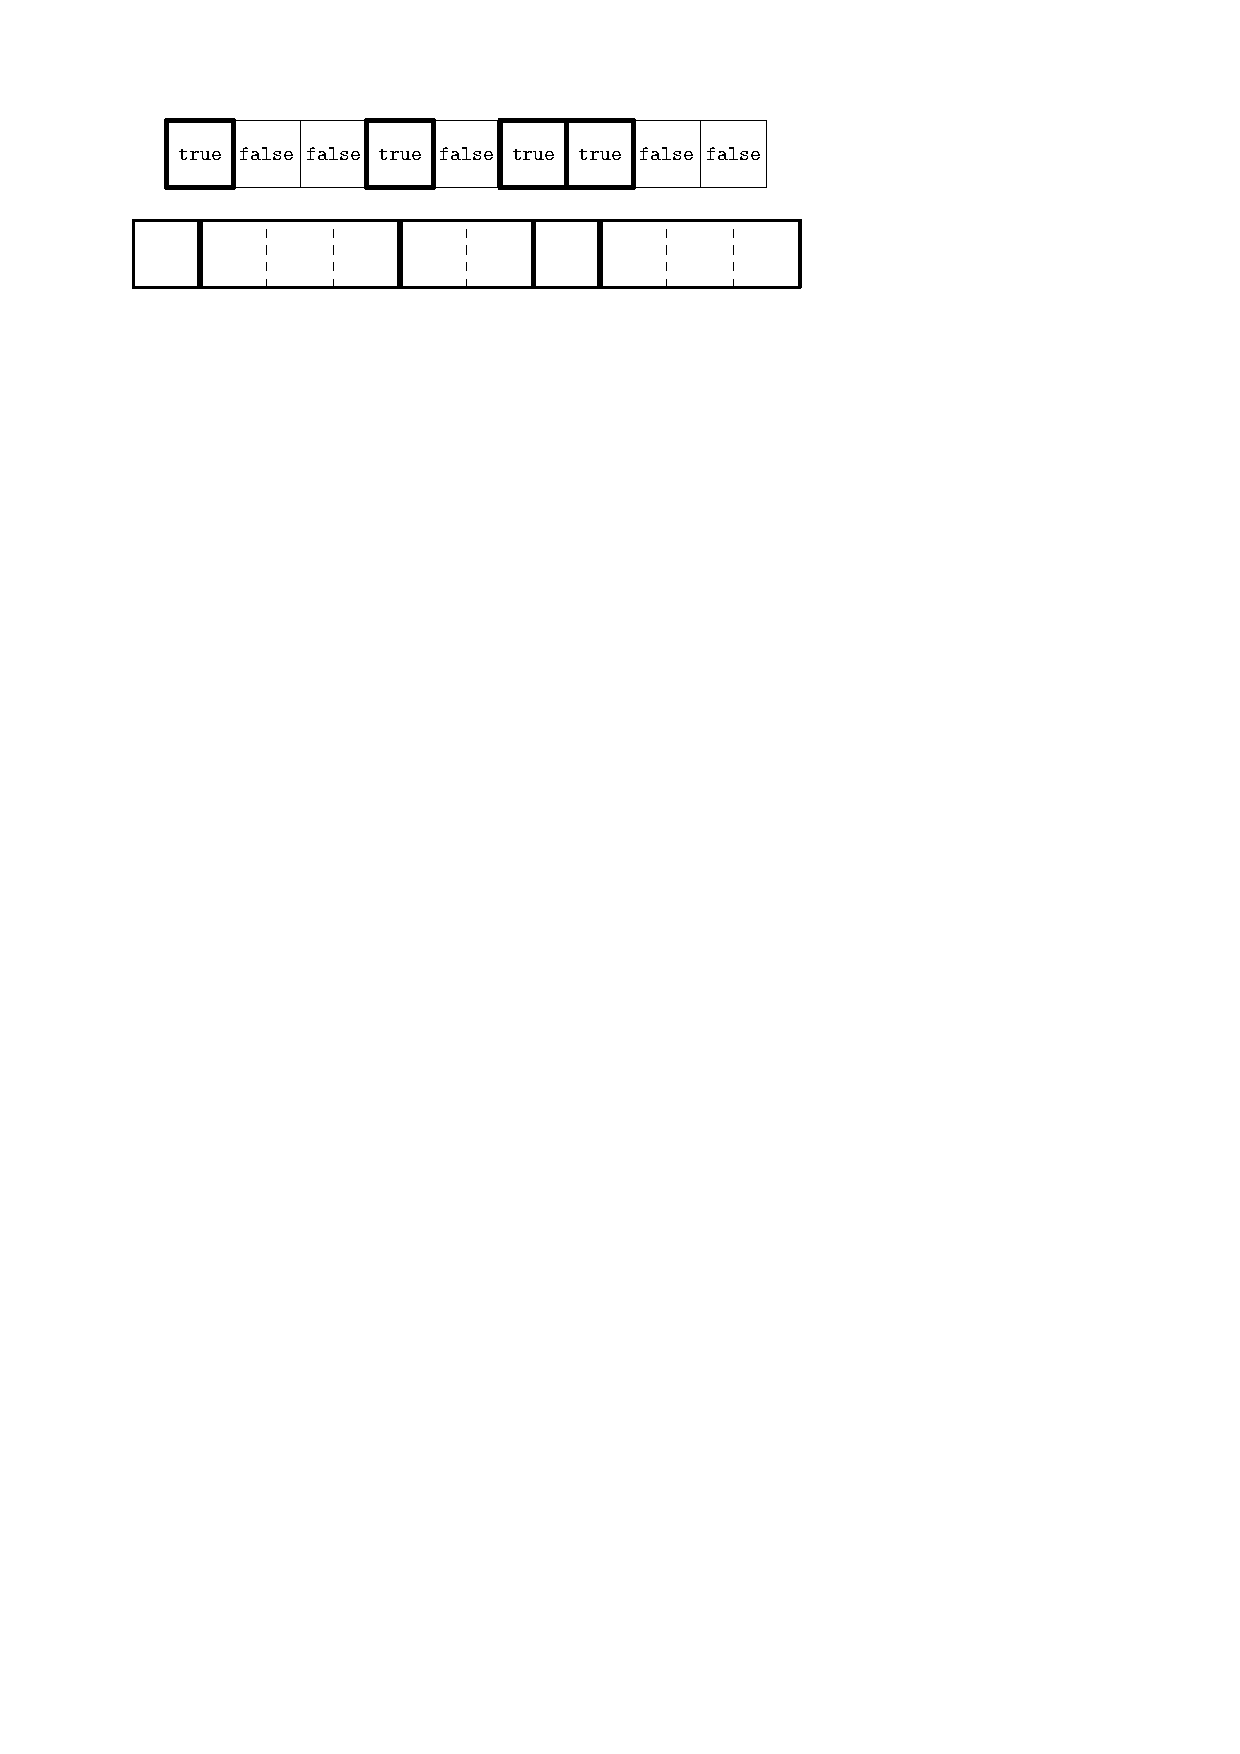
\includegraphics{../../Commun/Images/info-cours-algo-decoupe}\\
La découpe $1, 3, 2, 1, 3$ et le tableau de booléens correspondant.
\end{center}

\begin{questions}
\question Écrire une fonction \verb!decomposition(d: int, n: int) -> list[bool]!
  prenant en entrée un entier $n\in\N$ ainsi qu'un entier $d\in\interefo{0}{2^n}$,
  et renvoyant une liste de booléens $d_k$ de longueur $n$ telle que
  \[d=\sum_{k=0}^{n-1} d_k 2^k\]
  où le booléen \verb!True! représente le bit 1 et le booléen \verb!False! représente
  le bit 0.
\question Écrire une fonction \verb!prix_decoupe(d: list[bool], p: list[int]) -> int!
  prenant en entrée un tableau $d$ de longueur $n-1$ représentant une découpe d'une
  barre de longueur $n$, ainsi qu'un tableau $p$ de longueur $n+1$ représentant la
  liste des prix des différentes longueurs et renvoyant le prix de revente de la découpe
  $d$.
\question En déduire une fonction \verb!meilleur_prix(p: list[int]) -> tuple[list[bool], int]! renvoyant une meilleure découpe d'une barre de longueur $n$ ainsi que son prix
de revente correspondant.
\question Donner le prix ainsi qu'une découpe optimale associée pour l'exemple de tableau
  $p$ donné plus haut. 
\end{questions}

\emph{Nous verrons dans l'année des algorithmes dit de \og programmation dynamique \fg
permettant de résoudre ce type de problème plus efficacement.}
\magsubsection{Représentation mémoire des entiers non signés}


\magsubsection{Représentation mémoire des entiers signés}
\exercice{nom={Complément à 2}}
Dans une représentation en complément à 2 sur 8 bits, quels sont les entiers relatifs
représentés par $01101101$ et $10010010$~?

\exercice{nom={Machine 16~bits}}
On considère une architecture 16~bits. On considère les opérations
suivantes entre les entiers signés. Donner leur résultat mathématique
(en les considérant comme entiers naturels) puis leur résultat sur
16 bits signés.
\begin{questions}
\question $10\times 10$
\question $32767+1$
\question $256 \times (-256)$
\question $32767 - (-32768)$
\end{questions}

\magsection{Les nombres flottants}
\magsubsection{Représentation mémoire des flottants}

\exercice{nom={Le type float16}}
Dans le type \verb!float16! utilisé par Numpy, les nombres flottants sont représentés
sur 16 bits~: 1 bit pour le signe, 5 bits pour l'exposant, 10 bits pour la mantisse.
\begin{questions}
\question Donner la représentation machine dans de type de 1, de $-2$, puis du plus petit
  nombre strictement supérieur à 1, ainsi que se valeur.
\question Donner les représentations machine et la valeur des plus petits et des plus grands
  nombres normalisés.
\question Déterminer quel nombre est représenté par $0|01110|1001001000$.
\end{questions}

\magsubsection{Problèmes liés à l'arithmétique des nombres flottants}

\exercice{nom={Hamster jovial}}
  À votre grand bonheur, vous avez reçu pour Noël une balance d'excellente
  qualité : elle offre trois chiffres décimaux de précision, et ce autant
  pour des masses de l'ordre du gramme que de l'ordre de la tonne. Vous
  décidez d'utiliser cette balance pour mesurer la masse $m_h$ de votre
  hamster $h$. On suppose pour simplifier que $m_h$ est de l'ordre de
  100 grammes (un gros hamster, d'après Wikipedia).
  \begin{enumerate}
    \item Si $h$ accepte de monter docilement sur la balance et d'y rester
    le temps qu'elle fasse sa mesure, avec quelle précision obtiendrez-vous
    $m_h$ ?
    \item $h$, qui est d'une intelligence assez rare pour un rongeur,
    vous soupçonne, à tort ou à raison, de vouloir utiliser cette pesée pour
    justifier une mise au régime. Il descend donc immédiatement de la balance
    à chaque fois que vous l'y posez, et ce avant que la mesure n'ait été
    faite. Vous décidez alors de le peser indirectement : vous vous pesez une
    première fois avec $h$ dans la main, puis une deuxième fois sans $h$,
    et vous faites la différence. Avec quelle précision obtenez-vous $m_h$ ?
  \end{enumerate}

\exercice{nom={Ordre de sommation}}
On définit la suite $(u_n)$ par
\[\forall n\in\Ns\qsep u_n\defeq \sum_{k=2}^n \frac{1}{k(k-1)}.\]
\begin{questions}
\question En remarquant que
  \[\forall k\geq 2\qsep \frac{1}{k(k-1)}=\frac{1}{k-1} - \frac{1}{k},\]
  calculer explicitement $u_n$.
\question Afin de calculer $u_n$ à l'aide d'une somme, on écrit~:
\begin{pythoncodeline}
def sum_1(n):
    s = 0.0
    for k in range(2, n + 1):
        s = s + 1 / (k * (k - 1))
    return s
\end{pythoncodeline}
  Écrire le programme \verb!sum_2! calculant la même somme, mais sommant les $1/(k(k-1))$
  non pas avec $k$ allant de 2 à $n$ de manière croissante,d mais allant de $n$ à 2 de
  manière décroissante.
\question Comparer le résultat des deux fonctions précédentes pour $n = 10\ 000\ 000$.
  Quelle est la fonction la plus précise~? Comment expliquez-vous ce phénomène~?
\end{questions}


\magsection{Caractères et chaines de caractères}
\magsubsection{Codes Ascii et Unicode}
\magsubsection{Lecture et écriture dans un fichier}



% \begin{exoC}{}{}
%   On considère deux flottants $a$ et $b$ connus chacun avec $k$
%   chiffres significatifs (en base 10). On suppose que
%   $\abs{\frac{a - b}{a}} \simeq 10^{-d}$.
%   \begin{enumerate}
%     \item Que peut-on dire des $d$ chiffres les plus significatifs de $a$
%     et de $b$ ?
%     \item Combien y a-t-il de chiffres significatifs dans $a - b$ ?
%   \end{enumerate}
% \end{exoC}

% \begin{exemple}{}{}
%   \begin{multicols}{2}
%     On a :
%     \[
%       \frac{1-\cos(x)}{x^2} =
%       \frac 12 \left( \frac{ \sin \left( \frac x2\right)}{\frac x2}\right)^2
%       \Tend{x}{0} \frac 12
%     \]
%     et même plus précisément
%     \[
%       \abs{\frac{1 - \cos x}{x^2} - \frac 12} \Equiv{x}{0}
%       \frac{x^2}{24} \simeq \nombre{0,0417}\cdot x^2.
%     \]
%     Mais les deux expressions se comportent très différemment lors d'un calcul
%     en virgule flottante :
%     \begin{center}
%       \begin{tabular}{ccc}
%         \toprule
%         $x$ & $\abs{\frac{1-\cos(x)}{x^2} - \frac 12}$
%         &  $\abs{\frac 12 \left( \frac{ \sin \left( \frac x2\right)}{\frac x2}\right)^2
%           - \frac 12}$ \\
%         \otoprule
%         \py!1e-01! & \py!4.17e-04! & \py!4.17e-04! \\
%         \midrule
%         \py!1e-02! & \py!4.17e-06! & \py!4.17e-06! \\
%         \midrule
%         \py!1e-03! & \py!4.17e-08! & \py!4.17e-08! \\
%         \midrule
%         \py!1e-04! & \py!3.04e-09! & \py!4.17e-10! \\
%         \midrule
%         \py!1e-05! & \py!4.14e-08! & \py!4.17e-12! \\
%         \midrule
%         \py!1e-06! & \py!4.45e-05! & \py!4.17e-14! \\
%         \midrule
%         \py!1e-07! & \py!4.00e-04! & \py!4.44e-16! \\
%         \midrule
%         \py!1e-08! & \py!5.00e-01! & \py!0.00e+00! \\
%         \bottomrule
%       \end{tabular}
%     \end{center}
%   \end{multicols}
% \end{exemple}

% \subsubsection{Calcul de sommes}


%END_BOOK

\end{document}
